\documentclass[10pt]{article}
\usepackage{amsmath,amsthm,amssymb,dsfont,graphicx,xspace,epsfig,xcolor}
\usepackage{tikz, tkz-graph, tkz-berge}
\usetikzlibrary{decorations.pathreplacing}
\usetikzlibrary{patterns}
\usetikzlibrary{patterns.meta}
\usepackage{color}

\begin{document}

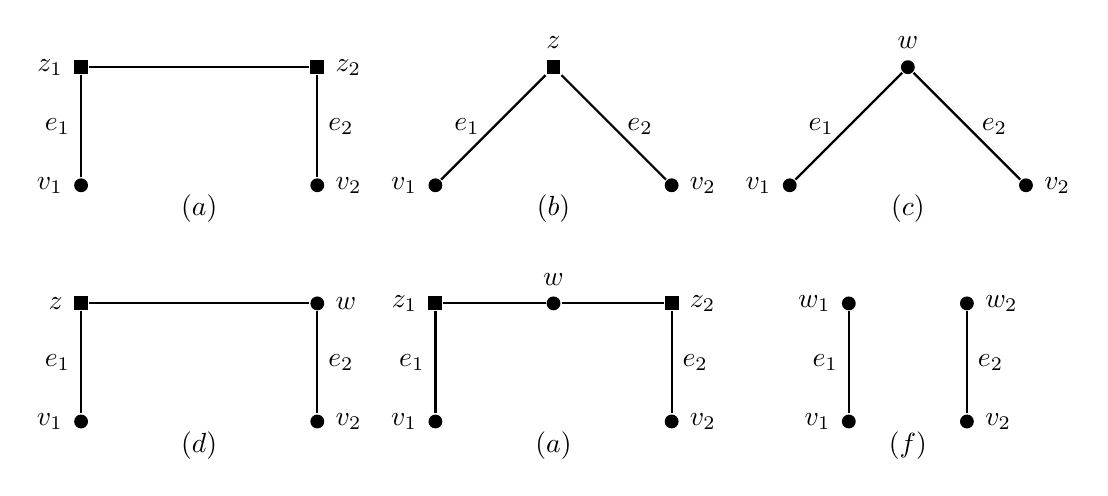
\begin{tikzpicture}[thick,scale=1, every node/.style={transform shape}]
        \tikzset{vertex/.style = {circle,fill=black,minimum size=5pt, inner sep=0pt}}
        \tikzset{squarevertex/.style = {rectangle,fill=black,minimum size=5pt, inner sep=0pt}}
        \tikzset{edge/.style = {->,> = latex'}}

        \begin{scope}
            \node[vertex, label=left:$v_1$] (v1) at (0, 0) {};
            \node[vertex, label=right:$v_2$] (v2) at (3, 0) {};
            \node[squarevertex, label=left:$z_1$] (z1) at (0, 1.5) {};
            \node[squarevertex, label=right:$z_2$] (z2) at (3, 1.5) {};
            \node[] (e1) at (-0.3,0.75) {$e_1$};
            \node[] (e2) at (3.3,0.75) {$e_2$};
            \node[] (a) at (1.5,-0.3) {$(a)$};
            \draw (v1) -- (z1) -- (z2) -- (v2);
        \end{scope}

        \begin{scope}[xshift=4.5cm]
            \node[vertex, label=left:$v_1$] (v1) at (0, 0) {};
            \node[vertex, label=right:$v_2$] (v2) at (3, 0) {};
            \node[squarevertex, label=above:$z$] (z) at (1.5, 1.5) {};
            \node[] (e1) at (0.4,0.75) {$e_1$};
            \node[] (e2) at (2.6,0.75) {$e_2$};
            \node[] (a) at (1.5,-0.3) {$(b)$};
            \draw (v1) -- (z) -- (v2);
        \end{scope}

        \begin{scope}[xshift=9cm]
            \node[vertex, label=left:$v_1$] (v1) at (0, 0) {};
            \node[vertex, label=right:$v_2$] (v2) at (3, 0) {};
            \node[vertex, label=above:$w$] (z) at (1.5, 1.5) {};
            \node[] (e1) at (0.4,0.75) {$e_1$};
            \node[] (e2) at (2.6,0.75) {$e_2$};
            \node[] (a) at (1.5,-0.3) {$(c)$};
            \draw (v1) -- (z) -- (v2);
        \end{scope}

        \begin{scope}[yshift=-3cm]
            \node[vertex, label=left:$v_1$] (v1) at (0, 0) {};
            \node[vertex, label=right:$v_2$] (v2) at (3, 0) {};
            \node[squarevertex, label=left:$z$] (z1) at (0, 1.5) {};
            \node[vertex, label=right:$w$] (z2) at (3, 1.5) {};
            \node[] (e1) at (-0.3,0.75) {$e_1$};
            \node[] (e2) at (3.3,0.75) {$e_2$};
            \node[] (a) at (1.5,-0.3) {$(d)$};
            \draw (v1) -- (z1) -- (z2) -- (v2);
        \end{scope}

        \begin{scope}[yshift=-3cm, xshift=4.5cm]
            \node[vertex, label=left:$v_1$] (v1) at (0, 0) {};
            \node[vertex, label=right:$v_2$] (v2) at (3, 0) {};
            \node[squarevertex, label=left:$z_1$] (z1) at (0, 1.5) {};
            \node[vertex, label=above:$w$] (w) at (1.5, 1.5) {};
            \node[squarevertex, label=right:$z_2$] (z2) at (3, 1.5) {};
            \node[] (e1) at (-0.3,0.75) {$e_1$};
            \node[] (e2) at (3.3,0.75) {$e_2$};
            \node[] (a) at (1.5,-0.3) {$(a)$};
            \draw (v1) -- (z1) -- (w) -- (z2) -- (v2);
        \end{scope}

        \begin{scope}[yshift=-3cm, xshift=9.75cm]
            \node[vertex, label=left:$v_1$] (v1) at (0, 0) {};
            \node[vertex, label=right:$v_2$] (v2) at (1.5, 0) {};
            \node[vertex, label=left:$w_1$] (w1) at (0, 1.5) {};
            \node[vertex, label=right:$w_2$] (w2) at (1.5, 1.5) {};
            \node[] (e1) at (-0.3,0.75) {$e_1$};
            \node[] (e2) at (1.8,0.75) {$e_2$};
            \node[] (a) at (0.75,-0.3) {$(f)$};
            \draw (v1) -- (w1);
            \draw (v2) -- (w2);
        \end{scope}

    \end{tikzpicture}

\end{document}